\documentclass[tikz,dvipsnames]{standalone}

\usetikzlibrary{shapes,decorations.markings}
\usetikzlibrary{decorations.pathmorphing,patterns}

\begin{document}

    \begin{minipage}{.45\textwidth}
    \centering
    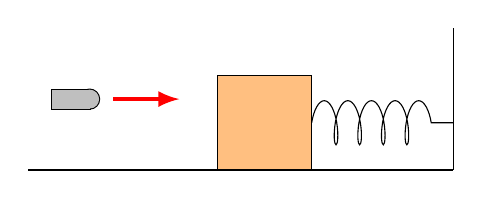
\begin{tikzpicture}[scale=1.2]
    \fill[orange!50] (0,0) rectangle (1,1) ;
    \draw (0,0) rectangle (1,1) ;
    \draw[-latex,red, ultra thick] (-1.1,0.75)--(-0.4,0.75);
    \draw[thick] (-1.75,0.65) rectangle (-1.75+0.4,0.65+0.2) ;
    \draw[thick] (-1.75+0.4,0.75) circle (0.1);
    \fill[gray!50] (-1.75,0.65) rectangle (-1.75+0.4,0.65+0.2) ;
    \fill[gray!50] (-1.75+0.4,0.75) circle (0.1);
    \draw[decoration={aspect=0.3, segment length=3mm, amplitude=2.8mm,coil},decorate] (1,0.5) -- (2.5,0.5); 
    \draw (-2,0)--(2.5,0); 
    \draw (2.5,1.5)--(2.5,0); 
    \end{tikzpicture}
    
    \end{minipage}
    \begin{minipage}{.45\textwidth}
    
   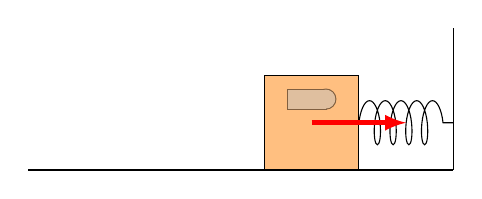
\begin{tikzpicture}[scale=1.2]
    \fill[orange!50] (0.5,0) rectangle (1.5,1) ;
    \draw[thick] (-1.75+2.5,0.65) rectangle (-1.75+0.4+2.5,0.65+0.2) ;
    \draw[thick] (-1.75+0.4+2.5,0.75) circle (0.1);
    \fill[gray!50] (-1.75+2.5,0.65) rectangle (-1.75+0.4+2.5,0.65+0.2) ;
    \fill[gray!50] (-1.75+0.4+2.5,0.75) circle (0.1);
    \draw[decoration={aspect=0.3, segment length=2mm, amplitude=2.8mm,coil},decorate] (1.5,0.5) -- (2.5,0.5); 
    \fill[orange!50,opacity=0.5] (0.5,0) rectangle (1.5,1) ;
    \draw (-2,0)--(2.5,0); 
    \draw (2.5,1.5)--(2.5,0);     
    \draw (0.5,0) rectangle (1.5,1) ;    
    \draw[-latex,red, ultra thick] (1,0.5)--(2,0.5);
    \end{tikzpicture}
    \end{minipage}

\end{document}